\documentclass[journal,12pt,twocolumn]{IEEEtran}
%
\usepackage{setspace}
\usepackage{gensymb}
\usepackage{xcolor}
\usepackage{caption}
%\usepackage{subcaption}
%\doublespacing
\singlespacing

%\usepackage{graphicx}
%\usepackage{amssymb}
%\usepackage{relsize}
\usepackage[cmex10]{amsmath}
\usepackage{mathtools}
%\usepackage{amsthm}
%\interdisplaylinepenalty=2500
%\savesymbol{iint}
%\usepackage{txfonts}
%\restoresymbol{TXF}{iint}
%\usepackage{wasysym}
\usepackage{hyperref}
\usepackage{amsthm}
\usepackage{mathrsfs}
\usepackage{txfonts}
\usepackage{stfloats}
\usepackage{cite}
\usepackage{cases}
\usepackage{subfig}
%\usepackage{xtab}
\usepackage{longtable}
\usepackage{multirow}
%\usepackage{algorithm}
%\usepackage{algpseudocode}
%\usepackage{enumerate}
\usepackage{enumitem}
\usepackage{mathtools}
%\usepackage{iithtlc}
%\usepackage[framemethod=tikz]{mdframed}
\usepackage{listings}
\let\vec\mathbf
\DeclarePairedDelimiter\abs{\lvert}{\rvert}%


%\usepackage{stmaryrd}


%\usepackage{wasysym}
%\newcounter{MYtempeqncnt}
\DeclareMathOperator*{\Res}{Res}
%\renewcommand{\baselinestretch}{2}
\renewcommand\thesection{\arabic{section}}
\renewcommand\thesubsection{\thesection.\arabic{subsection}}
\renewcommand\thesubsubsection{\thesubsection.\arabic{subsubsection}}

\renewcommand\thesectiondis{\arabic{section}}
\renewcommand\thesubsectiondis{\thesectiondis.\arabic{subsection}}
\renewcommand\thesubsubsectiondis{\thesubsectiondis.\arabic{subsubsection}}

%\renewcommand{\labelenumi}{\textbf{\theenumi}}
%\renewcommand{\theenumi}{P.\arabic{enumi}}

% correct bad hyphenation here
\hyphenation{op-tical net-works semi-conduc-tor}

\lstset{
language=Python,
frame=single, 
breaklines=true,
columns=fullflexible
}



\begin{document}
%

\theoremstyle{definition}
\newtheorem{theorem}{Theorem}[section]
\newtheorem{problem}{Problem}
\newtheorem{proposition}{Proposition}[section]
\newtheorem{lemma}{Lemma}[section]
\newtheorem{corollary}[theorem]{Corollary}
\newtheorem{example}{Example}[section]
\newtheorem{definition}{Definition}[section]
%\newtheorem{algorithm}{Algorithm}[section]
%\newtheorem{cor}{Corollary}
\newcommand{\BEQA}{\begin{eqnarray}}
\newcommand{\EEQA}{\end{eqnarray}}
\newcommand{\define}{\stackrel{\triangle}{=}}
\newcommand{\myvec}[1]{\ensuremath{\begin{pmatrix}#1\end{pmatrix}}}
\newcommand{\mydet}[1]{\ensuremath{\begin{vmatrix}#1\end{vmatrix}}}

\bibliographystyle{IEEEtran}
%\bibliographystyle{ieeetr}

\providecommand{\nCr}[2]{\,^{#1}C_{#2}} % nCr
\providecommand{\nPr}[2]{\,^{#1}P_{#2}} % nPr
\providecommand{\mbf}{\mathbf}
\providecommand{\pr}[1]{\ensuremath{\Pr\left(#1\right)}}
\providecommand{\qfunc}[1]{\ensuremath{Q\left(#1\right)}}
\providecommand{\sbrak}[1]{\ensuremath{{}\left[#1\right]}}
\providecommand{\lsbrak}[1]{\ensuremath{{}\left[#1\right.}}
\providecommand{\rsbrak}[1]{\ensuremath{{}\left.#1\right]}}
\providecommand{\brak}[1]{\ensuremath{\left(#1\right)}}
\providecommand{\lbrak}[1]{\ensuremath{\left(#1\right.}}
\providecommand{\rbrak}[1]{\ensuremath{\left.#1\right)}}
\providecommand{\cbrak}[1]{\ensuremath{\left\{#1\right\}}}
\providecommand{\lcbrak}[1]{\ensuremath{\left\{#1\right.}}
\providecommand{\rcbrak}[1]{\ensuremath{\left.#1\right\}}}
\providecommand{\rect}[1]{\text{rect}\ensuremath{\left(#1\right)}}
\providecommand{\sinc}[1]{\text{sinc}\ensuremath{\left(#1\right)}}
\theoremstyle{remark}
\newtheorem{rem}{Remark}
\newcommand{\sgn}{\mathop{\mathrm{sgn}}}
\providecommand{\res}[1]{\Res\displaylimits_{#1}} 
\providecommand{\norm}[1]{\lVert#1\rVert}
\providecommand{\mtx}[1]{\mathbf{#1}}
\providecommand{\fourier}{\overset{\mathcal{F}}{ \rightleftharpoons}}
\providecommand{\ztrans}{\overset{\mathcal{Z}}{ \rightleftharpoons}}

%\providecommand{\hilbert}{\overset{\mathcal{H}}{ \rightleftharpoons}}
%\providecommand{\system}{\overset{\mathcal{H}}{ \longleftrightarrow}}
\providecommand{\system}[1]{\overset{\mathcal{#1}}{ \longleftrightarrow}}
	%\newcommand{\solution}[2]{\textbf{Solution:}{#1}}
\newcommand{\solution}{\noindent \textbf{Solution: }}
\providecommand{\dec}[2]{\ensuremath{\overset{#1}{\underset{#2}{\gtrless}}}}
\numberwithin{equation}{section}
%\numberwithin{equation}{subsection}
%\numberwithin{problem}{subsection}
%\numberwithin{definition}{subsection}
\makeatletter
\@addtoreset{figure}{problem}
\makeatother

\let\StandardTheFigure\thefigure
%\renewcommand{\thefigure}{\theproblem.\arabic{figure}}
\renewcommand{\thefigure}{\theproblem}


%\numberwithin{figure}{subsection}

\def\putbox#1#2#3{\makebox[0in][l]{\makebox[#1][l]{}\raisebox{\baselineskip}[0in][0in]{\raisebox{#2}[0in][0in]{#3}}}}
     \def\rightbox#1{\makebox[0in][r]{#1}}
     \def\centbox#1{\makebox[0in]{#1}}
     \def\topbox#1{\raisebox{-\baselineskip}[0in][0in]{#1}}
     \def\midbox#1{\raisebox{-0.5\baselineskip}[0in][0in]{#1}}

\vspace{3cm}

\title{ 
%\logo{
%}
Fourier Series
%	\logo{Octave for Math Computing }
}
%\title{
%	\logo{Matrix Analysis through Octave}{\begin{center}\includegraphics[scale=.24]{tlc}\end{center}}{}{HAMDSP}
%}


% paper title
% can use linebreaks \\ within to get better formatting as desired
%\title{Matrix Analysis through Octave}
%
%
% author names and IEEE memberships
% note positions of commas and nonbreaking spaces ( ~ ) LaTeX will not break
% a structure at a ~ so this keeps an author's name from being broken across
% two lines.
% use \thanks{} to gain access to the first footnote area
% a separate \thanks must be used for each paragraph as LaTeX2e's \thanks
% was not built to handle multiple paragraphs
%

\author{ Varenya Upadhyaya} %<-this  stops a space

% note the % following the last \IEEEmembership and also \thanks - 
% these prevent an unwanted space from occurring between the last author name
% and the end of the author line. i.e., if you had this:
% 
% \author{....lastname \thanks{...} \thanks{...} }
%                     ^------------^------------^----Do not want these spaces!
%
% a space would be appended to the last name and could cause every name on that
% line to be shifted left slightly. This is one of those "LaTeX things". For
% instance, "\textbf{A} \textbf{B}" will typeset as "A B" not "AB". To get
% "AB" then you have to do: "\textbf{A}\textbf{B}"
% \thanks is no different in this regard, so shield the last } of each \thanks
% that ends a line with a % and do not let a space in before the next \thanks.
% Spaces after \IEEEmembership other than the last one are OK (and needed) as
% you are supposed to have spaces between the names. For what it is worth,
% this is a minor point as most people would not even notice if the said evil
% space somehow managed to creep in.



% The paper headers
%\markboth{Journal of \LaTeX\ Class Files,~Vol.~6, No.~1, January~2007}%
%{Shell \MakeLowercase{\textit{et al.}}: Bare Demo of IEEEtran.cls for Journals}
% The only time the second header will appear is for the odd numbered pages
% after the title page when using the twoside option.
% 
% *** Note that you probably will NOT want to include the author's ***
% *** name in the headers of peer review papers.                   ***
% You can use \ifCLASSOPTIONpeerreview for conditional compilation here if
% you desire.




% If you want to put a publisher's ID mark on the page you can do it like
% this:
%\IEEEpubid{0000--0000/00\$00.00~\copyright~2007 IEEE}
% Remember, if you use this you must call \IEEEpubidadjcol in the second
% column for its text to clear the IEEEpubid mark.



% make the title area
\maketitle

%\newpage

\tableofcontents

%\renewcommand{\thefigure}{\thesection.\theenumi}
%\renewcommand{\thetable}{\thesection.\theenumi}

\renewcommand{\thefigure}{\theenumi}
\renewcommand{\thetable}{\theenumi}

%\renewcommand{\theequation}{\thesection}


\bigskip

\begin{abstract}
This manual provides a simple introduction to Fourier Series
\end{abstract}
\section{Periodic Function}
Let 
\begin{align}
	x(t) &= A_0\abs{\sin\brak{2\pi f_0 t}}\label{eq:10-orig-diff-def}
\end{align}
\begin{enumerate}[label=\thesection.\arabic*
,ref=\thesection.\theenumi]
\item Plot $x(t)$.
\\\solution The following code plots Fig. \ref{fig:xt}
	\begin{lstlisting}
wget https://raw.githubusercontent.com/varenya27/EE3900/master/charger/codes/1_1.py
\end{lstlisting}
	\begin{figure}[h!]
	    \centering
	    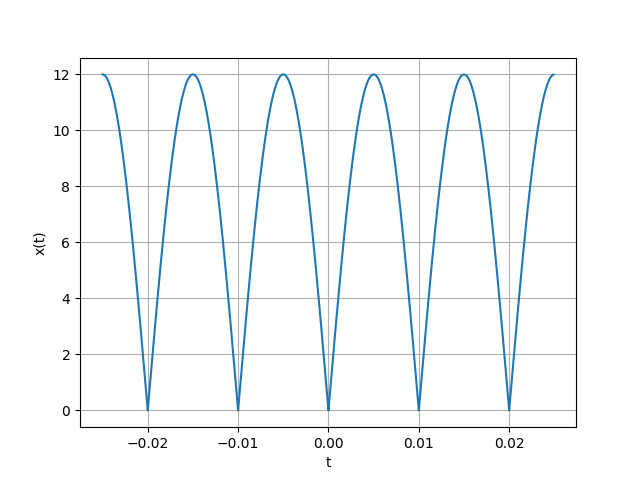
\includegraphics[width=\columnwidth]{figures/1_1.png}
	    \caption{x(t) }
	    \label{fig:xt}
	\end{figure}

\item Show that $x(t)$ is periodic and find its period.
Let T be the period of $x(t)$
\begin{align}
    x(t+T) &= A\abs{sin\brak{2\pi f_0\brak{t+T}}}\\
    &= A\abs{sin(2\pi f_0t+2\pi f_0T)}\\
    &= A\abs{\sin\brak{2\pi f_0 t}} \text,\quad 2\pi f_0T=\pi\\
    \implies T&= \frac{1}{2f_0}
\end{align}
\end{enumerate}
\section{Fourier Series}
Consider $A_0 =12$ and $f_0 = 50$ for all numerical calculations.
\begin{enumerate}[label=\thesection.\arabic*,ref=\thesection.\theenumi]
\item If
%\cite{proakis_dsp}
\begin{align}
	x(t) = \sum_{k = -\infty}^{\infty}c_ke^{\j2\pi kf_0 t}
\label{eq:one-Z-complex}
\end{align}
show that 
\begin{align}
	c_k = f_0\int_{-\frac{1}{2f_0}}^{\frac{1}{2f_0}}x(t)e^{-\j2\pi kf_0 t}\, dt
\label{eq:one-Z}
\end{align}
\\\solution \begin{align}
    	x(t) &= \sum_{k = -\infty}^{\infty}c_ke^{\j2\pi kf_0 t}\\
    	\int_{-\frac{1}{2f_0}}^{\frac{1}{2f_0}}x(t)e^{-\j2\pi nf_0 t}dt &= \int_{-\frac{1}{2f_0}}^{\frac{1}{2f_0}}\sum_{k = -\infty}^{\infty}c_ke^{\j2\pi \brak{k-n}f_0 t}dt\\
    	&= \sum_{k = -\infty}^{\infty}c_k\int_{-\frac{1}{2f_0}}^{\frac{1}{2f_0}}e^{\j2\pi \brak{k-n}f_0 t}dt\\
    	&= \sum_{k = -\infty}^{\infty}c_k \frac{1}{f_0}\delta(k-n)\\
    	&= \frac{1}{f_0}c_n\\
    	\implies c_n &= f_0\int_{-\frac{1}{2f_0}}^{\frac{1}{2f_0}}x(t)e^{-\j2\pi nf_0 t}\, dt
\end{align}
	\item Find $c_k$ for 
	\eqref{eq:10-orig-diff-def}\\\solution\begin{align}
	    c_k &= 50\int_{-0.01}^{0.01}12\abs{\sin\brak{2\pi 50t}}
    e^{-\j100\pi kt}\, dt \\
        &= 600\int_{-0.01}^{0.01}\abs{\sin\brak{100\pit}}
    \cos\brak{100\pi kt}\, dt \nonumber \\
        &+ \j 600\int_{-0.01}^{0.01}
        \abs{\sin\brak{100\pi t}}\sin\brak{100\pi kt}\, dt \\
        &= 600\int_{0}^{0.01}2\sin\brak{100\pi t}\cos\brak{100\pi kt}\, dt \\
        &= 600\int_{0}^{0.01}\brak{\sin\brak{100\pi\brak{k+1}t}}\, dt \nonumber \\ 
        &- 600\int_{0}^{0.01}\brak{\sin\brak{100\pi\brak{k-1}t}}\, dt \\ 
        &= 6\frac{1+\brak{-1}^k}{\pi}\brak{\frac{1}{k+1} - \frac{1}{k-1}} \\
        &= 
        \begin{cases}
            \frac{24}{\pi\brak{1-k^2}} & \text{even}\ k \\
            0 &  \text{odd} \ k
        \end{cases}
	\end{align}
\item Verify 
	\eqref{eq:one-Z-complex}
	using python.\\\solution The following code plots Fig. \ref{fig:xt-sim}
	\begin{lstlisting}
wget https://raw.githubusercontent.com/varenya27/EE3900/master/charger/codes/2_3.py
\end{lstlisting}
	\begin{figure}[h!]
	    \centering
	    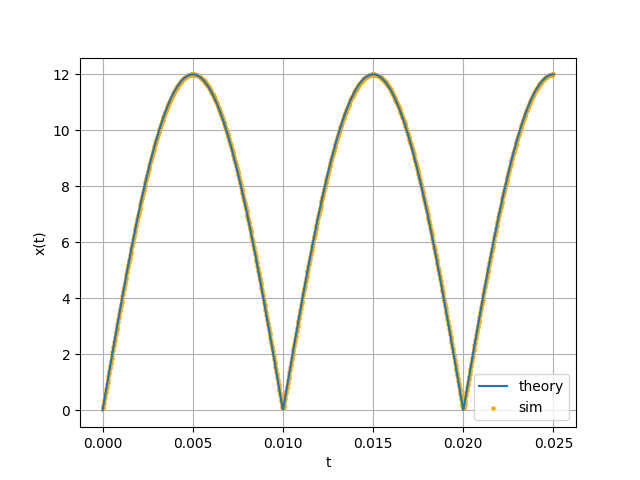
\includegraphics[width=\columnwidth]{figures/xt-sim.png}
	    \caption{x(t) from the fourier series}
	    \label{fig:xt-sim}
	\end{figure}
	\item Show that 
\begin{align}
	x(t) = \sum_{k = 0}^{\infty}\brak{a_k\cos{2\pi kf_0 t}+b_k\j\sin{2\pi kf_0 t}}
\label{eq:one-Z-real}
\end{align}
and obtain the formulae for $a_k$ and $b_k$.
\\\solution
\begin{align}
    x(t) &= \sum_{k = -\infty}^{\infty}c_ke^{\j2\pi kf_0 t} \\
         &= c_0 + \sum_{k = 1}^{\infty}c_ke^{\j2\pi kf_0t} + c_{-k}e^{-\j2\pi kf_0t} \\
         &= c_0 + \sum_{k = 1}^{\infty}\brak{c_k + c_{-k}}\cos\brak{2\pi kf_0t}  \nonumber \\
         &+ \sum_{k = 0}^{\infty}\j\brak{c_k - c_{-k}}\sin\brak{2\pi kf_0t}
\end{align}
Hence, for $k \ge 0$,
\begin{align}
    a_k &= 
    \begin{cases}
        c_0 & k = 0 \\
        c_k + c_{-k} & k > 0
    \end{cases} \label{eq:ak} \\
        &=
    \begin{cases}
        50\int_{-0.01}^{0.01}x(t)\, dt & k = 0 \\
        100\int_{-0.01}^{0.01}
        x(t)\cos\brak{100\pi kt}\, dt & k > 0
    \end{cases} \\
    b_k &= \frac{c_k - c_{-k}}{\j} = 100\int_{-0.01}^{0.01}
    x(t)\sin\brak{100\pi kt}\, dt
    \label{eq:bk}
\end{align}
\item Find $a_k$ and $b_k$ for 
	\eqref{eq:10-orig-diff-def}\\
\solution Clearly x(t) is even
\begin{align}
    x(t) &= \sum_{k = -\infty}^{\infty}c_ke^{\j2\pi kf_0 t} \\
          x(-t)&= \sum_{k = -\infty}^{\infty}c_ke^{-\j2\pi kf_0 t} \label{eq:sub} \\
          &= \sum_{k = -\infty}^{\infty}c_{-k}e^{\j2\pi kf_0 t}= x(t)\\
\implies c_k&= c_{-k}
\end{align}
thus for $k \ge 0$,
\begin{align}
    a_k &= 
    \begin{cases}
        \frac{24}{\pi} & k = 0 \\
        \frac{48}{\pi\brak{1 - k^2}} & k > 0,\ k\ \text{even} \\
        0 & \text{otherwise}
    \end{cases} \label{eq:ak-xt}\\
    b_k &= 0
    \label{eq:bk-xt}
\end{align}

	
\item Verify 
\eqref{eq:one-Z-real}
using python.
\\\solution The following code plots Fig. \ref{fig:xt-sim-ab}
	\begin{lstlisting}
wget https://raw.githubusercontent.com/varenya27/EE3900/master/charger/codes/2_6.py
\end{lstlisting}
	\begin{figure}[h!]
	    \centering
	    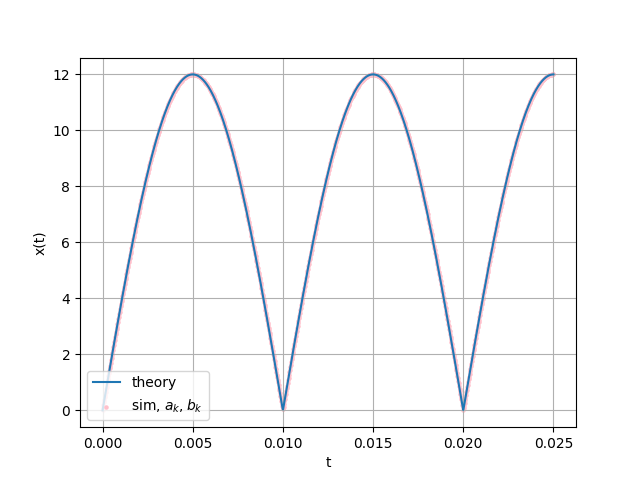
\includegraphics[width=\columnwidth]{figures/xt-sim-ab.png}
	    \caption{x(t) from the fourier series using $a_k, b_k$}
	    \label{fig:xt-sim-ab}
	\end{figure}
\end{enumerate}
\section{Fourier Transform}

 

\begin{enumerate}[label=\thesection.\arabic*
,ref=\thesection.\theenumi]
\item 
	\begin{align}
		\delta(t)&=0, \quad t\neq0
\\
		\int_{-\infty}^{\infty}\delta(t) \, dt&= 1
	\end{align}
 \item The Fourier Transform of $g(t)$ is
 \begin{align}
 G(f)=\int_{-\infty}^{\infty}g(t)e^{-j2\pi ft}\,dt
 \end{align}
 \item Show that 
 \begin{align}
	 g(t-t_0)&\system{F}G(f)e^{-j2\pi ft_0}\\
 \end{align}\\\solution\begin{align}
     g(t-t_0)&\system{F}\int_{-\infty}^{\infty}g(t-t_0)e^{-j2\pi ft}\,dt\\
     &= \int_{-\infty}^{\infty}g(t')e^{-j2\pi f\brak{t'+t_0}}\,dt'\\
     &= e^{-j2\pi ft_0}\int_{-\infty}^{\infty}g(t')e^{-j2\pi ft'}\,dt'\\
     &= G(f)e^{-j2\pi ft_0}
 \end{align}
 \item Show that 
 \begin{align}
	 G(t)&\system{F}g(-f)
 \end{align}\\\solution
 using the inverse fourier transform:
 \begin{align}
    g(t)&=\int_{-\infty}^{\infty}G(f)e^{j2\pi ft}\,df\\
    \implies g(f)&=\int_{-\infty}^{\infty}G(t)e^{j2\pi ft}\,dt\\
     \implies g(-f)&=\int_{-\infty}^{\infty}G(t)e^{-j2\pi ft}\,dt\\
     \implies G(t)&\system{F}g(-f)
 \end{align}
 \item $\delta(t)\system{F}?$\\\solution
 \begin{align}
     \delta(t)\system{F}&\int _{-\infty}^{\infty} \delta(t)e^{-j2\pi ft}\,dt\\
     &= 1
 \end{align}
 \item $e^{-j2\pi f_0t}\system{F}?$\\\solution
 \begin{align}
     e^{-j2\pi f_0t}\system{F}&\int _{-\infty}^{\infty} e^{-j2\pi f_0t}e^{-j2\pi ft}\,dt\\
     &= \int _{-\infty}^{\infty} e^{-j2\pi \brak{f+f_0}t}\,dt\\
     &= \delta(f+f_0)
 \end{align}
 \item $\cos(2\pi f_0t)\system{F}?$\\\solution
 \begin{align}
     \cos(2\pi f_0t)\system{F}&\int_{-\infty}^{\infty} \cos(2\pi f_0t)e^{-j2\pi ft}\,dt\\
     &= \frac{1}{2}\int_{-\infty}^{\infty} \brak{e^{2j\pi f_0t}+e^{-2j\pi f_0t}}e^{-j2\pi ft}\,dt\\
     &= \frac{1}{2}\brak{\delta(f-f_0) +\delta(f+f_0)}
 \end{align}
 \item Find the Fourier Transform of $x(t)$ and plot it.  Verify using python.\\\solution
 \begin{align}
     x(t)\system{F}&\int_{-\infty}^\infty\sum_{k=-\infty}^\infty c_k e^{-\j2\pi kf_0t}\,dt\\
     &= \sum_{k=-\infty}^\infty c_k \delta(kf_0+f)\\
     &= \sum_{k=-\infty}^\infty \frac{24}{\pi(1-4k^2)}\delta(2kf_0+f)
 \end{align}
 The following code plots Fig. \ref{fig:xt-ft}
	\begin{lstlisting}
wget https://raw.githubusercontent.com/varenya27/EE3900/master/charger/codes/3_8.py
\end{lstlisting}
	\begin{figure}[h!]
	    \centering
	    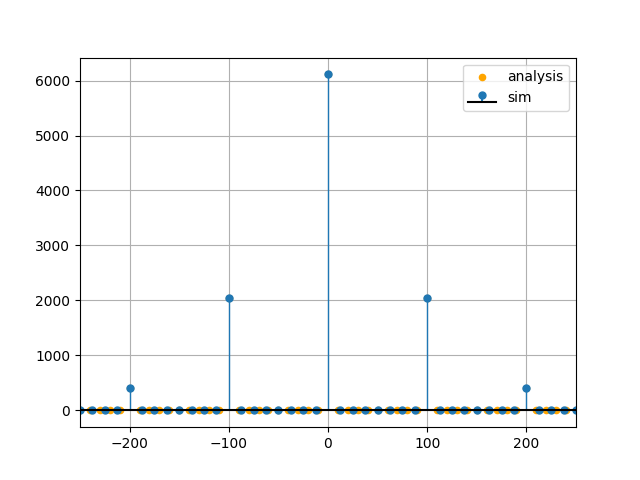
\includegraphics[width=\columnwidth]{figures/xt-ft.png}
	    \caption{fourier transform of $x(t)$ }
	    \label{fig:xt-ft}
	\end{figure}
 \item Show that 
 \begin{align}
	 \rect{t} \system{F} \sinc{t}
 \end{align}
 Verify using python.\\\solution
 \begin{align}
     \rect{t} \system{F}&\int_{-\infty}^\infty \rect{t}e^{-\j2\pi ft}\,dt\\
     &= \int_{-0.5}^{0.5}e^{-\j2\pi ft}\,dt\\
     &= \frac{\j}{2\pi f}\brak{e^{-\j\pi f}-e^{\j\pi f}}\\
     &= \frac{\sin{\pi f}}{\pi f}\\
     &= \sinc{f}
 \end{align}
  The following code plots Fig. \ref{fig:rect-ft}
	\begin{lstlisting}
wget https://raw.githubusercontent.com/varenya27/EE3900/master/charger/codes/3_9.py
\end{lstlisting}
	\begin{figure}[h!]
	    \centering
	    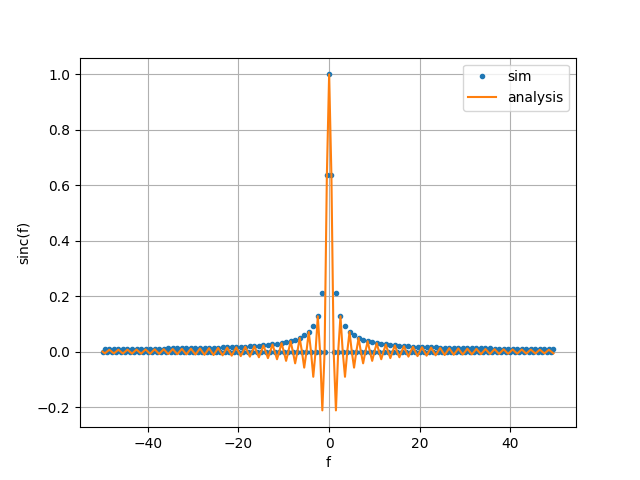
\includegraphics[width=\columnwidth]{figures/rect-ft.png}
	    \caption{fourier transform of $rect(t)$ }
	    \label{fig:rect-ft}
	\end{figure}

 \item 
$	 \sinc{t}\system{F} ?$.  Verify using python.
\\\solution Using the inverse fourier transform and the fact that $\rect{f}$ is even:
\begin{align}
    \sinc{t}\system{F}\rect{-f}=\rect{f}
\end{align}
  The following code plots Fig. \ref{fig:sinc-ft}
	\begin{lstlisting}
wget https://raw.githubusercontent.com/varenya27/EE3900/master/charger/codes/3_10.py
\end{lstlisting}
	\begin{figure}[h!]
	    \centering
	    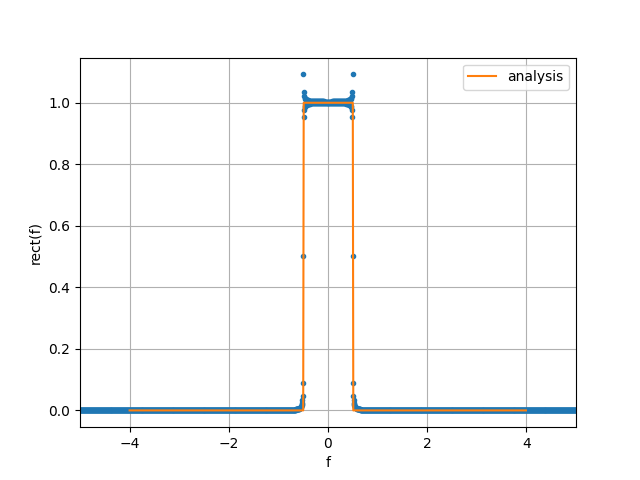
\includegraphics[width=\columnwidth]{figures/sinc-ft.png}
	    \caption{fourier transform of $sinc(t)$ }
	    \label{fig:sinc-ft}
	\end{figure}
\end{enumerate}
\section{Filter}
\begin{enumerate}[label=\thesection.\arabic*
,ref=\thesection.\theenumi]
\item Find $H(f)$ which transforms $x(t)$ to DC 5V.\\\solution Let $y(t)$ represent the 5V DC output. $H(f)$ should be a low pass (to ensure DC) filter. With $f_0 = 50Hz$:
\begin{align}
    H(f) &= \rect{\frac{f}{2f_0}}
\end{align}
Since the output is 5V
\begin{align}
    \frac{24}{\pi}H(f) &= 5\rect{\frac{f}{2f_0}}\\
    &= \frac{5\pi}{24}\rect{\frac{f}{2f_0}}
\end{align}
\item Find $h(t)$.
Applying the inverse fourier transform:
\begin{align}
    h(t) &= \int_\infty^\infty H(f)e^{\j2\pi ft}\,df\\
    &= \frac{5\pi}{24}\int_\infty^\infty \rect{\frac{f}{2f_0}}e^{\j2\pi ft}\,df\\
    &= \frac{5\pi f_0}{12}\sinc{2f_0t}
\end{align}
\item Verify your result using  through convolution.
  The following code plots Fig. \ref{fig:conv-ft}
	\begin{lstlisting}
wget https://raw.githubusercontent.com/varenya27/EE3900/master/charger/codes/4_3.py
\end{lstlisting}
	\begin{figure}[h!]
	    \centering
	    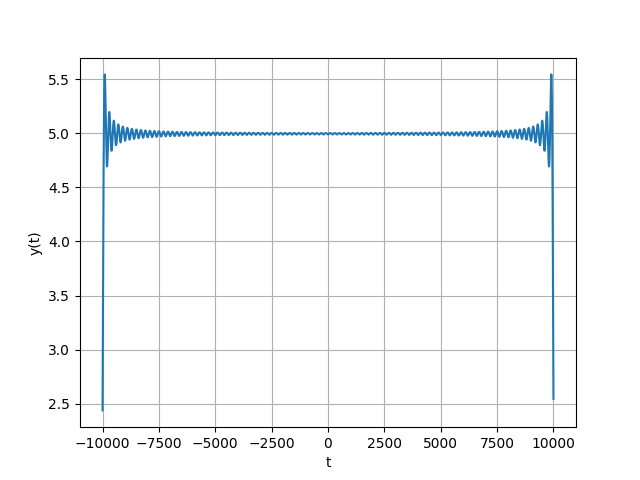
\includegraphics[width=\columnwidth]{figures/conv-hx.png}
	    \caption{convolution of $h(t)$ and $x(t)$ }
	    \label{fig:conv-ft}
	\end{figure}

\end{enumerate}
\section{Filter Design}
\begin{enumerate}[label=\thesection.\arabic*
,ref=\thesection.\theenumi]
\item Design a Butterworth filter for $H(f)$.
\item Design a Chebyschev filter for $H(f)$.
\item Design a circuit for your Butterworth filter.
\item Design a circuit for your Chebyschev filter.
\end{enumerate}


\end{document}